\subsubsection{NATaS}
\`A la différence des autres ordonnanceurs, NATaS va tenir compte de l'affinité NUMA des tâches.
%
Cette affinité a été définit par Taggre de tel sorte à équilibrer la charge sur les différents bancs NUMA.
%
NATaS offre de meilleurs performances sur Rostand par rapport à la politique d'allocation interleave.
%
La factorisation est 40\% plus rapide avec 8 variables primaires et la résolution triangulaire est 23\% plus rapide.
%
Avec 1 variable primaire nous n'obtenons pas de gain sur la résolution triangulaire.


%   (-_-)   %
\begin{figure}[!h]
     \begin{center}
        \subfigure[Factorisation ILU(0).]{
          \label{fig:res_facto_nas_rostand}
          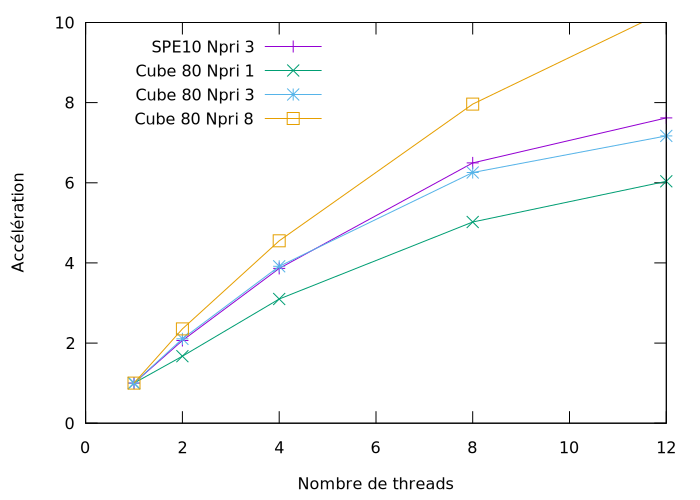
\includegraphics[width=0.48\textwidth]{res_facto_nas}
        }
        \subfigure[Résolution triangulaire]{
          \label{fig:res_trsv_nas_rostand}
          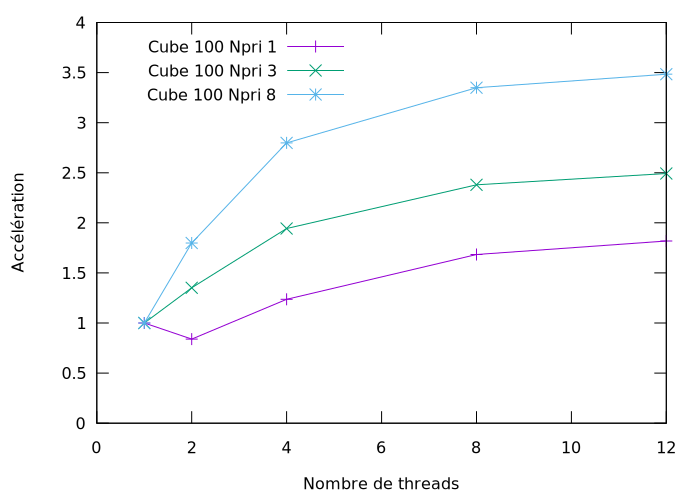
\includegraphics[width=0.48\textwidth]{res_trsv_nas}
        }
    \end{center}
    \caption{Performances sur Rostand avec NATaS.}
\end{figure}



%   (-_-)   %
\begin{figure}[!h]
     \begin{center}
        \subfigure[Factorisation ILU(0).]{
          \label{fig:res_facto_nas_manu}
          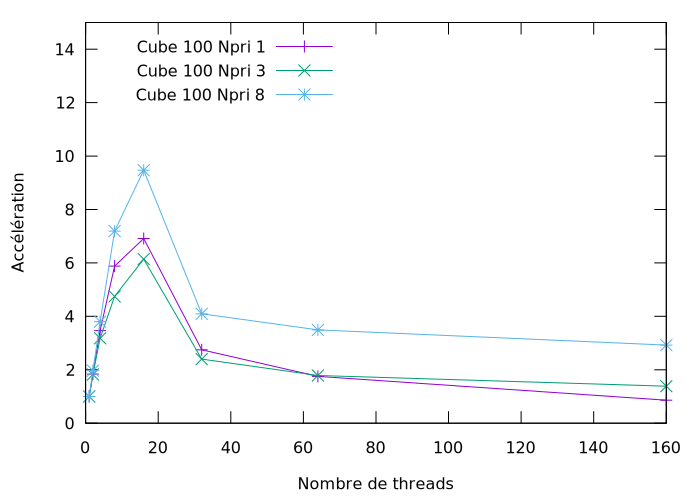
\includegraphics[width=0.48\textwidth]{res_facto_nas_manu}
        }
        \subfigure[Résolution triangulaire]{
          \label{fig:res_trsv_nas_manu}
          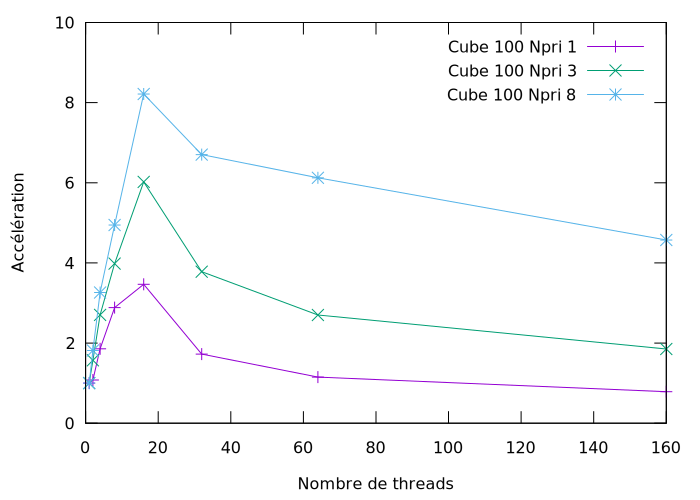
\includegraphics[width=0.48\textwidth]{res_trsv_nas_manu}
        }
    \end{center}
    \caption{Performances sur Manumanu avec NATaS.}
\end{figure}
